\section{目的}
依 Lab 14（PDF 58--61 頁）比較靜態 CMOS 反相器與六電晶體 Schmitt trigger，研究正回授尺寸對遲滯、雜訊與延遲的影響，並加入不同架構。

\section{Spec 對照}
\begin{longtable}{p{0.31\linewidth}p{0.29\linewidth}p{0.31\linewidth}}
\toprule
講義要求（PDF頁） & 實作 & 驗證與界線 \\\midrule
步驟 1：圖 14.1 三種 feedback、雙向 DC（58--59、61） & 01\_hysteresis 六案例 & 獨立掃描，避免同時跳支路 \\
步驟 2：雜訊容忍（59--61） & 02\_noise\_immunity & 相同有限時間擾動比較 \\
步驟 3：速度比較（60--61） & 03\_delay\_comparison & 相同 8 fF 與輸入邊緣 \\
問題：另一架構三種比較（61） & ALT；05\_alternative\_dc & DC、noise、delay 皆有 \\
額外數值核對 & 04\_slow\_ramp\_check & 1/10 $\mu$s 斜坡對 DC \\
\bottomrule
\end{longtable}


\section{電路與設計推導}
主串聯 PMOS 各 $3.6/0.25\,\mu$m，NMOS 各 $1.2/0.25\,\mu$m；feedback PMOS/NMOS 依三個案例為 $1.8/0.6$、$3.6/1.2$、$5.4/1.8\,\mu$m，L 皆 0.25。保留圖 14.1 的交叉回授接法。比較用 INV 為 $1.8/0.6\,\mu$m。替代架構使用一個強輸入反相器（$W_p/W_n=3.6/1.2$）驅動兩個弱交叉耦合反相器（各 $1.8/0.6$），也是六個 MOS，但回授拓樸不同。

上掃輸入令輸出降至一半的點為 $V^+$，下掃為 $V^-$，遲滯寬度 $H=V^+-V^-$。它是有記憶的雙分支特性，不應直接套單值 inverter 的兩個 unity-gain noise margins。講義公式是平方律近似；本次沒有可獨立驗證的內部 $V_T$ 與 mobility，不把它當精確設計方程。

\section{模擬設定}
本次為使用另行提供模型的教學改寫，電源為 1.0 V、溫度為 $25\,^{\circ}\mathrm C$。保留講義指定的拓樸、負載及比較尺寸；原講義的 2.5 V 製程結果不是本次模型的驗收數值。1 V 僅是模擬條件，不能視為模型的安全額定。所有 MOS 的 Bulk 明確接至相應電源軌。

HSPICE S-2021.09 使用 RUNLVL=6；保存波形、列印資料及原生量測。圖表由本次數據重繪；CSV 保存於各 Lab 的 results。完成模擬表示求解成功，並不代表製程可靠度已驗證。加密模型仍有被抑制的警告；既有診斷未取得可判讀的進一步內容，因此不宣稱警告無害或全部模型限制已滿足。

DC 0--1 V／1--0 V、0.5 mV。原始多個 .dc 指令會忽略預期的反向替換，已用起迄與步距參數明確建立雙向案例。另發現多個遲滯元件並列時 Newton 分支跳轉互相影響，故 DC 改單一 feedback 案例；慢斜坡以 1 與 10 $\mu$s/V 雙向暫態驗證。雜訊刺激同 Lab8，delay 比較使用 0.1 ns 邊緣、8 fF 輸出負載，50\% crossing 量傳播延遲。

\section{結果與規格檢查}
五份 deck、12 個案例皆完成。下表門檻單位 V；ramp 採較慢的 10 $\mu$s/V。
\begin{center}\small
\begin{tabular}{llllll}
\toprule
Circuit & $V^+_{DC}$ & $V^-_{DC}$ & $H_{DC}$ & $V^+_{ramp}$ & $V^-_{ramp}$ \\
\midrule
SCH 1 & 0.5922 & 0.3968 & 0.1955 & 0.5928 & 0.3961 \\
SCH 2 & 0.6332 & 0.3573 & 0.2760 & 0.6341 & 0.3564 \\
SCH 3 & 0.6552 & 0.3353 & 0.3200 & 0.6565 & 0.3338 \\
Alt & 0.6321 & 0.0879 & 0.5441 & 0.6325 & 0.0873 \\
\bottomrule
\end{tabular}
\end{center}

\begin{figure}[htbp]
\centering
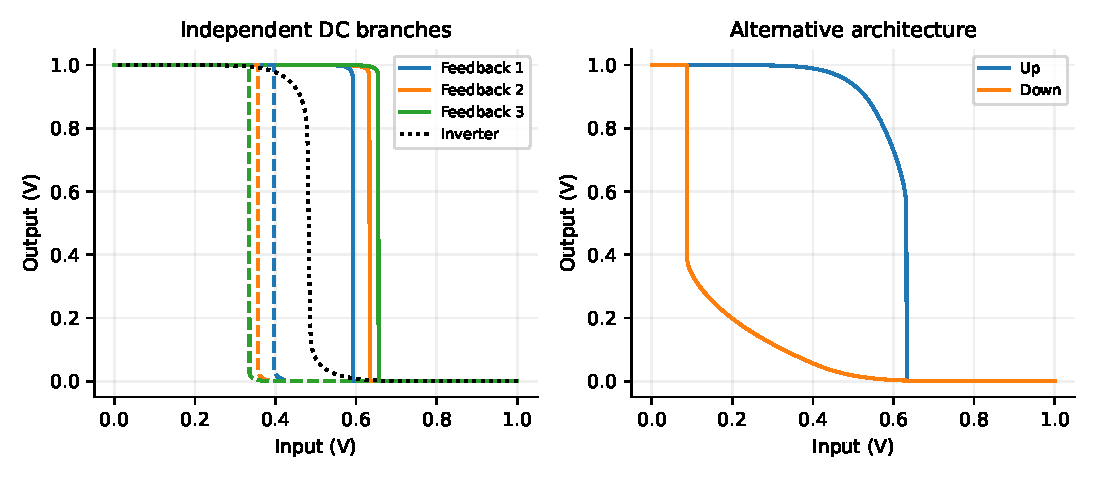
\includegraphics[width=\linewidth]{figures/schmitt_hysteresis.pdf}
\caption{三種回授及替代架構的獨立 DC 遲滯；由本次 HSPICE 數據重繪。}
\end{figure}
\begin{center}\small
\begin{tabular}{lllll}
\toprule
Circuit & $t_r$ (ps) & $t_f$ (ps) & $t_{pHL}$ (ps) & $t_{pLH}$ (ps) \\
\midrule
INV & 106.95 & 51.92 & 63.86 & 88.77 \\
SCH 1 & 219.10 & 84.35 & 149.36 & 203.59 \\
SCH 2 & 260.52 & 101.05 & 196.67 & 230.75 \\
SCH 3 & 301.50 & 118.33 & 244.97 & 256.13 \\
Alt & 427.75 & 106.61 & 70.70 & 311.56 \\
\bottomrule
\end{tabular}
\end{center}

\begin{figure}[htbp]
\centering
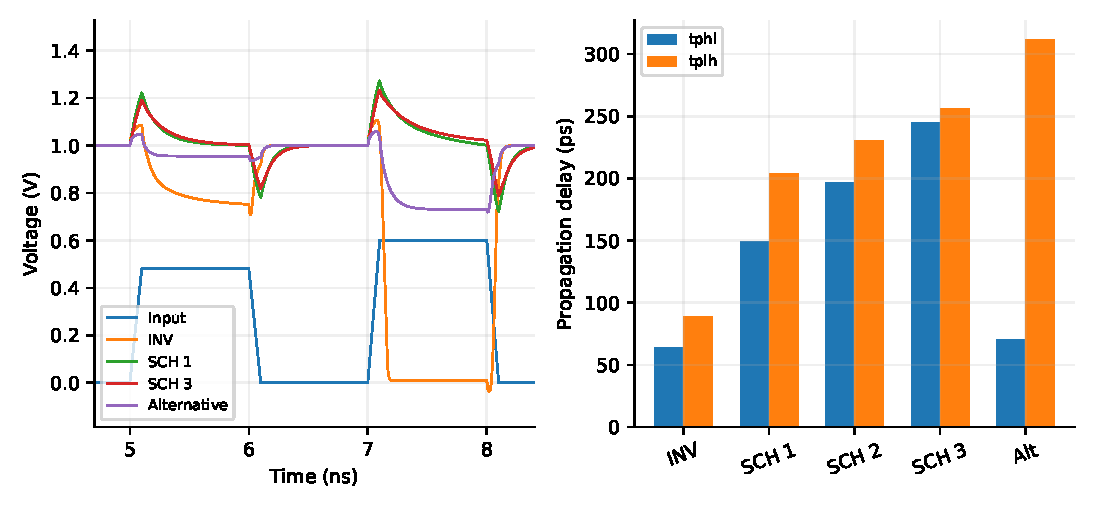
\includegraphics[width=\linewidth]{figures/schmitt_noise_delay.pdf}
\caption{有限時間雜訊及相同負載的傳播延遲；由本次 HSPICE 數據重繪。}
\end{figure}


\section{討論}
加大回授使 DC 遲滯由約 0.195 增至 0.320 V，同時增加延遲。較慢斜坡對獨立 DC 的最大門檻差約 1.5 mV；這是有限速度與數值收斂的檢查，並非完全零速證明。0.6 V、0.9 ns 的擾動可使 INV 翻轉，Schmitt 在此時間窗仍可能保持原狀；接近 DC 門檻的短脈衝可因有限再生時間未完成切換，不能據此宣稱 DC 容限大於量得門檻。實際資料也含短暫超電源軌的電壓，未驗證其可靠度。

替代架構的遲滯約 0.544 V，但下降輸入門檻僅約 0.088 V，對兩種雜訊不對稱，且上升輸出較慢；因此「更大遲滯」不等於全面較佳。增加 feedback 的好處需與速度、恢復條件與輸入負載一起評估。

\section{結論}
三個步驟與替代架構問題均完成 DC、暫態及數值交叉檢查；強回授的速度代價與替代架構的不對稱均據實列出。原講義的電壓值及未驗證的模型可靠度沒有被視為已滿足。
